% !TeX spellcheck = en_US

\chapter{Introduction}

% study computer science, (theoretical informatics), automata theory, value of this theory

Automata theory is recommended as part of a standard computer science curriculum~\cite[pp. 5-6]{GI16}. As other such theories it provides the chance to gain a precise cognitive model yielding new perspectives on problems and givens. This may thus lead to increased problem solving skills and more accurate thinking.

% typical topic - minimization, (why typical)

A typical task in automata theory is the minimization of a given deterministic finite automaton (DFA). The classic textbook ``Introduction to automata theory, languages, and computation'' by Hopcroft et. al.~\cite{HMU01} presents a practicable minimization algorithm. In this work we will confine ourselves to look at DFA minimizations using that algorithm.

% sketch situation

In an introduction course to theoretical computer science minimization tasks are thus likely to occur in supplementary exercises or exams. As of the creation of such tasks, one may assume, that it is done mostly manually. Automation would yield here the following advantages:

\begin{itemize}
	\item freeing time for other things, e.g. research, helping students face-to-face, designing the whole exercise sheet
	
	\item generation of tasks which lie in a well-defined range
	
	\item increased predictability and consistency of the generated task properties, which can be adjusted accurately through various parameters
	
	\item saves human operators from the generating task which involves monotonous work
\end{itemize}
\gregor{Delete or find extern from wikipedia}
Engagement on this topic promises moreover increased clarification which kind of minimization tasks can be generated, and where difficulties of those tasks lie.

This work aims to provide theoretical foundations for a DFA minimization task generator. What requirements a user has towards such a program will be discussed in a short requirements analysis. Based on this work a DFA minimization generator has been implemented. It can be found at \url{https://github.com/bt701607/Generation-of-DFA-Minimization-Problems}.

\section{Preliminaries}

We start with defining preliminary theoretical foundations.

\subsection{Deterministic Finite Automatons}

A 5-tuple $A = (Q, \Sigma, \delta, s, F)$ with $Q$ being a finite set of \emph{states}, $\Sigma$ a finite set of \emph{alphabet symbols}, $\delta \colon\ Q \times \Sigma \to Q$ a \emph{transition function}, $s \in Q$ a \emph{start state} and $F \subseteq Q$ \emph{final states} is called \emph{deterministic finite automaton} (DFA)~\cite[p. 46]{HMU01}. From now on $\mathfrak{A}$ shall denote the set of all DFAs.

We say $\delta(q,\sigma) = p$ is a transition from $q$ to $p$ using symbol $\sigma$. We define the \emph{extended transition function} $\delta^* : Q \times \Sigma^* \to Q$ of a DFA $A = (Q, \Sigma, \delta, s, F)$ as:
\begin{itemize}
	\item $\delta^*(q,\varepsilon) = q$
	\item $\delta^*(q,w\sigma) = \delta(\delta^*(q,w),\sigma)$ for all $q \in Q$, $w \in \Sigma^*$, $\sigma \in \Sigma$
\end{itemize}
Then, the \emph{language} of that DFA is defined as $L(A) = \{\ w\ |\ \delta^*(w) \in F\ \}$~\cite[pp. 49-50. 52]{HMU01}.

Given a state $q \in Q$. With $d^-(q)$ we denote the set of all \emph{ingoing} transitions $\delta(q', \sigma) = q$ of $q$. With $d^+(q)$ we denote the set of all \emph{outgoing} transitions $\delta(q, \sigma) = q'$ of $q$~\cite[pp. 2-3]{CP05}. If a transition is of the form $\delta(q, \sigma) = q$, then we say that $q$ has a \emph{loop}.

\begin{definition}\label{ch:1:unreachable-states}
	We say a state $q$ is \emph{(un-)reachable} in a DFA $A$, iff there is (no) a word $w \in \Sigma^*$ such that $\delta^*(s, w) = q$.
\end{definition}
\noindent If all states of a DFA $A$ are reachable, then we say $A$ is \emph{accessible}~\cite[p. 2]{CP05}.

A DFA is called \emph{complete} iff for all states, every symbol of the alphabet is used on an outgoing transition: $\forall q\in Q\colon \forall\sigma\in\Sigma\colon \exists p\in Q\colon \delta(q,\sigma) = p$. Note, that every incomplete DFA can be converted to a complete one by adding a so called \emph{dead state}~\cite[p. 67]{HMU01}. The resulting automaton has the same language.

\begin{figure}
	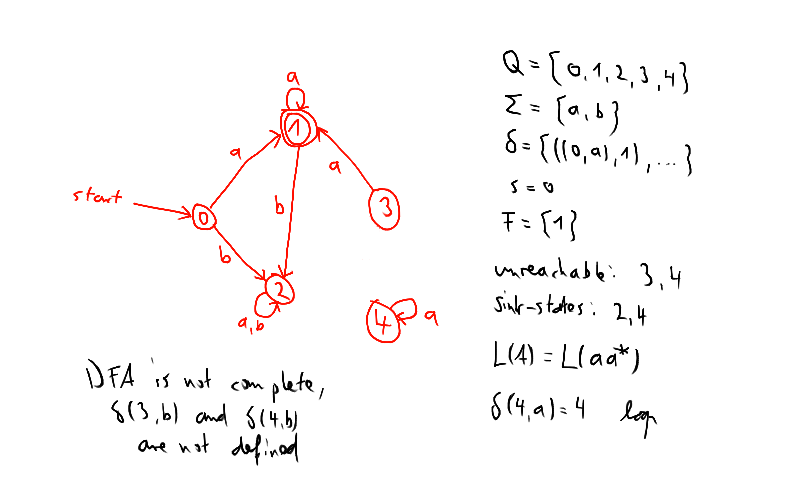
\includegraphics[width=\linewidth]{images/dfa.png}
	\caption{An example DFA and its properties.}
	\label{fig:dfa}
\end{figure}

\subsection{Minimal DFAs}

This section closely follows~\cite[pp. 42-45]{Sch01}. We call a DFA $A$ \emph{minimal}, if there exists no other automaton with the same language using less states. With $\mathfrak{A}_{min}$ we shall denote the set of all minimal DFAs.

The \emph{Nerode-relation} $\equiv_L\ \subseteq\ \Sigma^* \times \Sigma^*$ of a language $L$ with alphabet $\Sigma$ is defined as follows:
\begin{displaymath}
	x \equiv_L y\ \Leftrightarrow_{def}\ \forall z\in\Sigma^*\colon (xz\in L \Leftrightarrow yz\in L)
\end{displaymath}
The Nerode-relation of a DFA $A$ is the the Nerode-relation of its language: $\equiv_{L(A)}$. If the context makes it clear, than we will shorten the notation of a equivalence class $[x]_{\equiv_L}$ with $[x]$.

The \emph{equivalence class automaton} $A_L = (Q_L, \Sigma_L, \delta_L, s_L, F_L)$ to a regular language $L$ with alphabet $\Sigma$ is defined as follows:
\begin{itemize}
	\item $Q_L = \{\ [x]\ |\ x \in \Sigma^*\ \}$
	\item $\Sigma_L = \Sigma$
	\item $\delta_L([x], \sigma) = [x\sigma],\ \forall x\in\Sigma^*,\ \forall\sigma\in\Sigma$
	\item $s = [\varepsilon]$
	\item $F = \{\ [x]\ |\ x \in L\ \}$
\end{itemize}
\begin{theorem}
	Given a language $L$, then the equivalence class automaton $A_L$ is minimal.
\end{theorem}

\subsection{Practical Isomorphy of DFAs}

Given two DFAs $A_1 = (Q_1, \Sigma_1, \delta_1, s_1, F_1)$ and $A_2 = (Q_2, \Sigma_2, \delta_2, s_2, F_2)$. We say $A_1$ and $A_2$ are \emph{practical isomorph}, iff:
\begin{itemize}
	\item $|Q_1| = |Q_2|$, $|\Sigma_1| = |\Sigma_2|$ and
	\item there exists a bijection $\phi\colon \Sigma_1 \to \Sigma_2$ such that:
	\item there exists a bijection $\pi\colon Q_1 \to Q_2$ such that:
	
	$\pi(s_1) = s_2$
	
	$\forall q\in Q_1\colon (q\in F_1 \Longleftrightarrow \pi(q)\in F_2)$
	
	$\forall q\in Q_1\colon \forall\sigma\in\Sigma_1\colon \pi(\delta_1(q,\sigma))=\delta_2(\pi(q),\phi(\sigma)))$
\end{itemize}
Note that practical isomorphy between two DFAs $A_1, A_2$ does not imply $L(A_1) = L(A_2)$. This would be given, if $\Sigma_1 = \Sigma_2$ were the case (see~\cite[p. 45]{Sch01}). However the language of such DFAs is equivalent except for an exchange of alphabet symbols:
\[
	\{\ \phi(\sigma_0)\ldots\phi(\sigma_n)\ |\ \sigma_0\ldots\sigma_n\in L(A_1)\ \} = L(A_2)
\]
Practical isomorphy will be sufficient for our case. \gregor{why?}
%\begin{theorem} \textnormal{\cite[p. 45]{Sch01}} 
%	Every minimal DFA is unique except for isomorphy.
%\end{theorem}
%So it
%\begin{corollary}\label{ch:1:cor:all-min-dfa-ism}
%	Every minimal DFA $A$ is isomorph to its corresponding equivalence class automaton $A_{L(A)}$.
%	\gregor{All min. DFAs are ism. to each other, including A\_L}
%\end{corollary}
\gregor{Write down isomorphism test. Maybe discuss faster methods here? Look for faster methods in general?}

\subsection{Equivalent and distinguishable state pairs}

\begin{definition}[Equivalent and Distinguishable State Pairs]\cite[p. 154]{HMU01}
	A state pair $q_1, q_2 \in Q$ of a DFA $A = (Q, \Sigma, \delta, s, F)$ is called \emph{equivalent}, iff $\sim_A(q_1, q_2)$ is true, whereas
	\begin{displaymath}
	q_1\ \sim_A\ q_2 \Leftrightarrow_{def}\ \forall z \in \Sigma^* \colon\ (\delta^*(q_1, z) \in F \Leftrightarrow \delta^*(q_2, z) \in F)
	\end{displaymath}
	If $q_0 \not\sim_A q_1$, then $q_0$ and $q_1$ are called a \emph{distinguishable} state pair. The relation $\sim_A$ is an equivalence relation
\end{definition}
%\noindent Note the similarity between $\equiv_{L(A)}$ and $\sim_A$.:
%\begin{align*}
%	x\ \equiv_{L(A)}\ y\ \Leftrightarrow&\ \forall z\in\Sigma^*\colon (xz \in L \Leftrightarrow yz \in L) \\
%	& \\
%	q_1\ \sim_A\ q_2\ \Leftrightarrow&\ \forall z \in \Sigma^* \colon\ (\delta^*(q_1, z) \in F \Leftrightarrow \delta^*(q_2, z) \in F)
%\end{align*}
%We will prove the following statement regarding both relations:
%\begin{proposition}[Relationship of $\equiv_{L(A)}$ and $\sim_A$] \label{ch:1:prop-ner-eq} $ $ \\
%    \[
%    	x \equiv_{L(A)} y\ \Leftrightarrow\ \delta^*(s,x)=q_1\ \land\ \delta^*(s,y)=q_2\ \land\ q_1 \sim_A q_2
%    \]
%\end{proposition}
%\noindent Informally said: $x \equiv_{L(A)} y$ is true if and only if $q_1 \sim_A q_2$ whereas $q_1, q_2$ are reachable via $x,y$.
%\begin{proof} Via direct proof.
%    \begin{align*}
%    \ \delta^*(s,x)=q_1 \land \delta^*(s,y)=q_2\ \land\ & q_1 \sim_A q_2 \\
%    \Leftrightarrow\ \delta^*(s,x)=q_1 \land \delta^*(s,y)=q_2\ \land\ &(\forall z \in \Sigma^* \colon\ \delta^*(q_1, z) \in F \Leftrightarrow \delta^*(q_2, z) \in F) \\
%    \Leftrightarrow\hspace{5.65cm}&\ \forall z \in \Sigma^* \colon\ \delta^*(\delta^*(s,x), z) \in F \Leftrightarrow \delta^*(\delta^*(s,y), z) \in F \\
%    \Leftrightarrow\hspace{5.65cm}&\ \forall z \in \Sigma^* \colon\ \delta^*(s,xz) \in F \Leftrightarrow \delta^*(s,yz) \in F \\
%    \Leftrightarrow\hspace{5.65cm}&\ \forall z \in \Sigma^* \colon\ xz \in L(A) \Leftrightarrow yz \in L(A) \\
%    \Leftrightarrow\hspace{5.65cm}& x \equiv_{L(A)} y
%    \end{align*}
%\end{proof}
%\begin{corollary}
%    If the DFA $A$ is accessible, then there exists a $1:1$-correspondence between the equivalence classes of $\equiv_{L(A)}$ and $\sim_A$.
%\end{corollary}

%\noindent Proposition~\ref{ch:1:prop-ner-eq} can be supplemented by an even stronger declaration. Towards this declaration we first define, analogous to the equivalence class automaton, the \emph{$\sim$-equivalence automaton} $A_{\sim_A} = (Q_{\sim_A}, \Sigma_{\sim_A}, \delta_{\sim_A}, s_{\sim_A}, F_{\sim_A})$ to a DFA $A$:
%\begin{itemize}
%    \item $Q_{\sim_A} = \{[q]_{\sim_A} | q \in Q\}$
%    \item $\Sigma_{\sim_A} = \Sigma$
%    \item $\delta_{\sim_A}([q]_{\sim_A}, \sigma) = [\delta(q, \sigma)]_{\sim_A}, \forall q \in Q, \sigma \in \Sigma$
%    \item $s_{\sim_A} = [s]_{\sim_A}$
%    \item $F_{\sim_A} = \{[q]_{\sim_A} | q \in Q\}$
%\end{itemize}

%\begin{theorem}
%    If the DFA $A$ is accessible, then $A_{\sim_A}$ is minimal and thus isomorph to $A_L$.
%\end{theorem}

\subsection{The minimization algorithm}

This minimization algorithm \MinAlg\ works in four major steps, removing essentially states in such a way, that no unreachable states and no equivalent state pairs are left.
\begin{enumerate}
	\item Compute all unreachable states via breadth-first search.
	
	\vspace{0.2cm}
	\begin{algorithmic}[1]
		\Function{\CompUnr}{$A$}
			\State $U \gets Q \setminus \{s\}$	\Comment{undiscovered states}
			\State $O \gets \{s\}$				\Comment{observed states}
			\State $D \gets \{\}$				\Comment{discovered states}
			\While {$|O| > 0$}
				\State $N \gets \{\ p\ | \ \exists q \in O\ \sigma \in \Sigma \colon\ \delta(q, \sigma) = p\ \land\ p \notin O \cup D\ \}$
				\State $U \gets U \setminus N$
				\State $D \gets D \cup O$
				\State $O \gets N$
			\EndWhile
			\State \Return $U$
		\EndFunction
	\end{algorithmic}

	\item Remove all unreachable states and their transitions.
	
	\vspace{0.2cm}
	\begin{algorithmic}[1]
		\Function{\RemUnr}{$A, U$}
            \State $\delta' \gets \delta \setminus \{\ ((q,\sigma),p)\ |\ q\in U\ \lor\ p\in U\ \}$
			\State \Return $(Q \setminus U, \Sigma, \delta', s, F \setminus U)$
		\EndFunction
	\end{algorithmic}

	\item Compute all equivalent state pairs ($\sim_A$). Inspired by Schöning~\cite[p. 46]{Sch01} \gregor{And TI-VL}.
	
	\vspace{0.2cm}
	\begin{algorithmic}[1]
		\Function{\CompDist}{$A$} \label{ch:1:minmark}
		\State $M \gets \{ (p,q), (q,p)\ |\ p \in F, q \notin F \}$
		\Do
			\State $M' \gets \{ (p,q)\ |\ (p,q) \notin M \land \exists \sigma \in \Sigma \colon (\delta(p,\sigma), \delta(q,\sigma)) \in M \}$
			\State $M \gets M \cup M'$
		\doWhile {$M' \neq \emptyset$}
		\State \Return $Q^2 \setminus M$
		\EndFunction
	\end{algorithmic}
	Note that \CompDist\ requires its input automaton to be complete. \gregor{Why?}

	\item Merge all equivalent state pairs, which are exactly those in $\sim_A$. Inspired by Högberg~\cite[p. 10]{HL20}.
	
	\vspace{0.2cm}
	\begin{algorithmic}[1] \label{ch:1:minmerge}
		\Function{\RemEq}{$A$, $\sim_A$} \Comment{$[\cdot]_{\sim_A}$ shall be abbreviated $[\cdot]$}
            \State $Q_E \gets \emptyset$
            \State $\delta_E \gets \emptyset$
            \State $F_E \gets \emptyset$
            \For {$q$ \textbf{in} $Q$}
                \State Add $[q]$ to $Q_E$
                \For {$\sigma$ \textbf{in} $\Sigma$}
                    \State $\delta_E([q], \sigma) = [\delta(q, \sigma)]$
                \EndFor
                \If {$q \in F$}
                    \State Add $[q]$ to $F_E$
                \EndIf
            \EndFor
			\State \Return $(Q_E, \Sigma, \delta_E, [s], F_E)$
		\EndFunction
	\end{algorithmic}
	Note that \RemEq\ creates complete automatons.
\end{enumerate}

\vspace{0.2cm}
\begin{algorithmic}[1] \label{ch:1:minalg}
    \Function{\MinAlg}{$A_{task}$}
    \State $A_{re} \gets \RemUnr(A_{task}, \CompUnr(A_{task}))$
    \State $A_{sol} \gets \RemEq(A_{re}, \CompDist(A_{re}))$
    \State \Return $A_{sol}$
    \EndFunction
\end{algorithmic}
\vspace{0.2cm}
\noindent This DFA minimization algorithm has been found by Hopcroft~\cite{Hop71} and was established in teaching by Hopcroft et al.~\cite[pp. 154-164]{HMU01}.

\begin{theorem}\label{ch:1:min-alg-correct}\textnormal{\cite[pp. 162-164]{HMU01}}
	\MinAlg\ computes a minimal DFA to its input DFA.
\end{theorem}

\subsection{$m$-\CompDist.}

When looking at \CompDist, one notes, that it computes distinct subsets of $Q \times Q$ on the way. Indeed, one could write the algorithm in such a way, that these subsets are explicitly computed in form of a function $m\colon\mathbb{N}\to\mathcal{P}(Q\times Q)$:
\vspace{0.2cm}
\begin{algorithmic}[1] \label{ch:1:m-minmark}
	\Function{$m$-\CompDist}{$A$}
	\State $i \gets 0$
	\State $m(0) \gets \{ (p,q), (q,p)\ |\ p \in F, q \notin F \}$
	\Do
		\State $i \gets i + 1$
		\State $m(i) \gets \{ (p,q), (q,p)\ |\ (p,q) \notin \bigcup{m(\cdot)} \land \exists \sigma \in \Sigma \colon (\delta(p,\sigma), \delta(q,\sigma)) \in m(i-1) \}$
	\doWhile {$m(i) \neq \emptyset$}
	\State \Return $\bigcup{m(\cdot)}$
	\EndFunction
\end{algorithmic}
\vspace{0.2cm}
Using this redefinition, we can easier refer to the state pairs marked in a certain iteration. We will use both variants in exchange.

We will denote the number of iterations done by \CompDist\ on an DFA $A$ as $\mmD(A)$. Note that $\mmD(A) = \max n \in \mathbb{N}\ |\ m(n) \neq \emptyset$. \gregor{Does that note maybe fit very well to the proof of lemma~\ref{ch:3:semantics-of-D(A)}?}

%\subsection{\MinAlg-partition of a DFA}
%
%When looking at \MinAlg, one may note, that we can partition the states $Q_A$ of any DFA $A$ into three parts:
%\begin{itemize}
%	\item a subset of \emph{unreachable} states $U_A = \{\ u_1, \ldots, u_{\mathcal{Q}_{unr}}\ \}$ of size $\mathcal{Q}_{unr}$, found and removed in step 1 and 2
%	\item a subset of \emph{redundant} states $R_A = \{\ r_1, \ldots, r_{\mathcal{Q}_{eq}}\ \}$ of size $\mathcal{Q}_{eq}$, found and removed in step 3 and 4
%	\item a subset of \emph{essential} states $E_A = \{\ e_1, \ldots, e_\mathcal{Q}_{sol}\ \}$ of size $\mathcal{Q}_{sol}$, which are left over after applying the algorithm
%\end{itemize}
%Note that the set of essential states to a DFA is dependent on the implementation of \RemEq, but we know, that there will always be states left over, and for a given DFA the number will always be the same \gregor{why}.

%\gregor{Example: In~\ref{fig:dfa_ex_task} and~\ref{fig:dfa_ex_sol} the state pairs $(A,D), (C,E)$ are equivalent and all others distinguishable. The states $A, G, C, B$ are essential, for they show up in the minimized automaton. The states $D, E$ are therefore redundant.}

\subsection{Another equivalence automaton}

Consider step 3 and 4 of \MinAlg. A view on these algorithms reveal, that they are essentially collapsing each $\sim$-equivalence class of a DFA $A$ into one state.

\begin{definition}[$\sim_A$-equivalence automaton] \label{ch:1:sim-eq-dfa}
    We will call the automaton $E_A = (Q_E, \Sigma_E, \delta_E, s_E, F_E)$ created by \CompDist\ and \RemEq($A$)\ the \emph{$\sim_A$-equivalence automaton} of $A$. It has the following properties:
    \begin{itemize}
        \item $Q_E = \{\ [q]\ |\ q \in Q\ \}$
        \item $\Sigma_E = \Sigma$
        \item $\delta_E([q], \sigma) = [\delta(q, \sigma)], \forall q \in Q, \sigma \in \Sigma$
        \item $s_E = [s]_\sim$
        \item $F_E = \{\ [q]\ |\ q \in Q\ \}$
    \end{itemize}
    Note, that we know by theorem~\ref{ch:1:min-alg-correct} that $E_A$ is guaranteed to be a minimal automaton to $A$, if $A$ has no unreachable states.
\end{definition}

%Note moreover that, since $A_{sol}$ is minimal, there exists an isomorphism renaming $e_1,\ldots,e_\mathcal{Q}_{sol}$ such that they correspond to the equivalence classes of $\equiv_{L(A_{task})}\ = \ \equiv_{L(A_{re})}$ and $\sim_{A_{re}}$.
%
%However there might exist no isomorphism connecting $e_1,\ldots,e_\mathcal{Q}_{sol}$ and the equivalence classes of $\sim_{A_{task}}$, since possible unreachable states might form $\sim$-equivalence classes that are distinct to those of the reachable states.

\section{Requirements analysis}

Now that we have introduced all necessary basic definitions, we shall do a short analysis of an example DFA minimization task and its sample solution, as it could have been given to students in an introductory course to automata theory.

\subsection{Example of a DFA minimization task for students}

\gregor{search for typical task in standard text books}

\begin{figure}
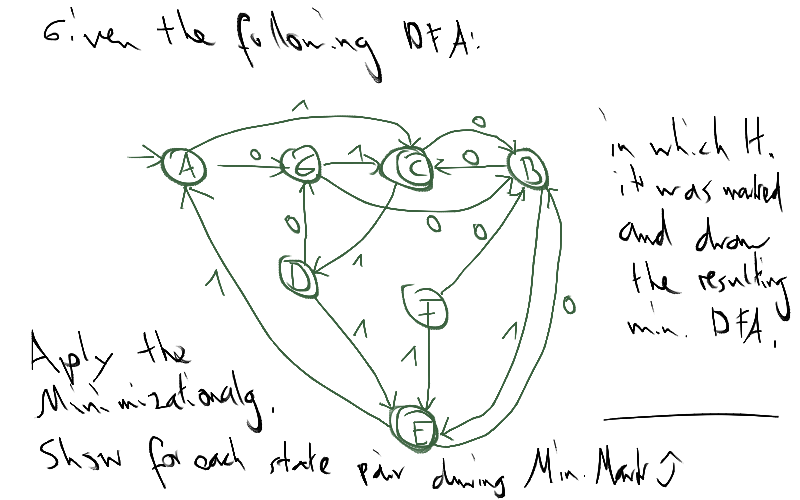
\includegraphics[width=\linewidth]{images/dfa_ex_task.png}
\caption{An example DFA minimization task.}
\label{fig:dfa_ex_task}
\end{figure}

\begin{figure}
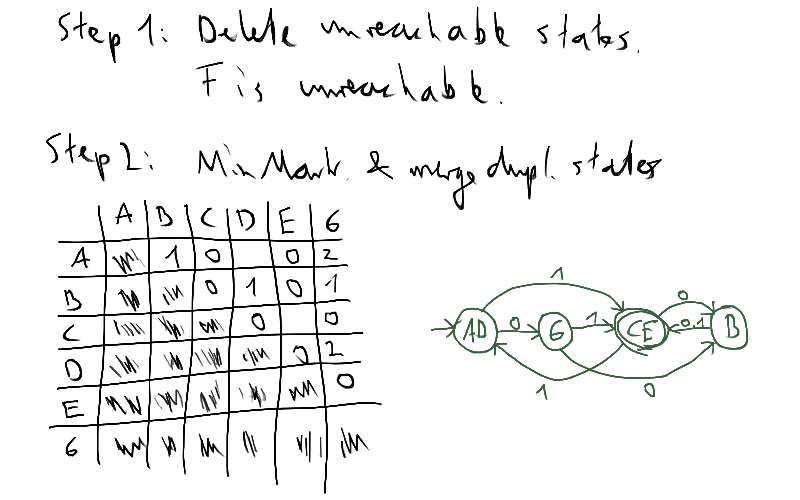
\includegraphics[width=\linewidth]{images/dfa_ex_sol.png}
\caption{Solution to the DFA minimization task in fig.~\ref{fig:dfa_ex_task}.}
\label{fig:dfa_ex_sol}
\end{figure}

\noindent Figures~\ref{fig:dfa_ex_task} and~\ref{fig:dfa_ex_sol} show such a task and solution. The students are confronted with a \emph{task DFA} $A_{task}$. Firstly, unreachable states have to be eliminated, we then gain the \emph{reachable DFA} $A_{re}$. Secondly equivalent state pairs of $A_{re}$ are merged such that the minimal \emph{solution DFA} $A_{sol}$ is found. The table $T$ displayed in figure~\ref{fig:dfa_ex_sol} is nothing else but a visualization of the function $m$, whereas $T(q_0, q_1) = i \Leftrightarrow (q_0, q_1) \in m(i)$.

We do some rather formal statements and requirements. Firstly, we can state that
\begin{itemize}
	\item $A_{re} = \RemUnr(A_{task}, \CompUnr(A_{task}))$ and
	\item $A_{sol} = \RemEq(A_{re}, \CompDist(A_{re}))$
\end{itemize}
Therefore $A_{sol}$ is minimal regarding $A_{re}$ and $A_{task}$. Secondly the languages of $A_{task}, A_{re}$ and $A_{sol}$ are be equal. We know that \CompDist\ requires $A_{re}$ to be complete and that \RemEq\ creates complete DFAs, so $A_{sol}$ is complete too. Furthermore we know that every state of $A_{re}$ is reachable since it is the output of \RemUnr.

\gregor{How to define 'already found DFA sol' as requirement. Final states argument missing.}

\subsection{Difficulty adjustment possibilities}

Concerning the execution of \MinAlg\ we find that its difficulty can be classified through various classification numbers.

\paragraph*{\CompDist-depth ($\mmD(A_{task})$).}

Consider the computation of the sets $m(i)$ in \CompDist. Determining $m(0)$ is quite straightforward, because it consists simply of tests whether two states are in $F \times Q \setminus F$ (see~\ref{ch:1:m-minmark}, line 3). Determining $m(1)$ is less easy: The rule for determining all $m(i), i > 0$ is different to that for $m(0)$ and more complicated (see~\ref{ch:1:m-minmark}, line 6). Determining $m(2)$ requires the same rule. It shows nonetheless a students understanding of the terminating behavior of \CompDist: It does not stop after computing $m(1)$, but only when no more distinguishable state pairs were found. Concerning the sets $m(i), i > 2$ however no additional understanding can be shown.

It would therefore be sensible if $\mmD(A_{task})$ could be adjusted for example by parameters $m_{min}, m_{max}$ which give lower and upper bounds for that value.

\paragraph*{Number of states ($\mathcal{Q}_{sol}, \mathcal{Q}_{eq}, \mathcal{Q}_{unr}$).}

To control the number of states in $A_{task}, A_{re}$ and $A_{sol}$, we will introduce three parameters: $\mathcal{Q}_{sol}, \mathcal{Q}_{eq}, \mathcal{Q}_{unr} \in \mathbb{N}$. These parameters get their meaning by the following equations:
\begin{align*}
    |Q_{sol}| &= \mathcal{Q}_{sol} \\
    |Q_{re}| &= \mathcal{Q}_{sol} + \mathcal{Q}_{eq} \\
    |Q_{task}| &= \mathcal{Q}_{sol} + \mathcal{Q}_{eq} + \mathcal{Q}_{unr}
\end{align*}
It is sensible to have $\mathcal{Q}_{unr} > 1, \mathcal{Q}_{eq} > 1$, such that \RemUnr\ and \RemEq\ will not be skipped. To not make the task trivial, $\mathcal{Q}_{sol} > 2$ is sensible. An exercise instructor will find it useful, to control exactly how big $\mathcal{Q}_{unr}$, $\mathcal{Q}_{eq}$ and $\mathcal{Q}_{sol}$ are: The higher $\mathcal{Q}_{unr}, \mathcal{Q}_{eq}$, the more states have to be eliminated and merged. The higher $\mathcal{Q}_{sol} + \mathcal{Q}_{eq}$, the more state pairs have to be checked during \CompDist.

\gregor{Concept for min max.}
%To control the number of states in $A_{task}, A_{re}$ and $A_{sol}$, we will introduce three pairs of parameters, denoting each ranges: $Q_{s,min}, Q_{s,max}$ for the number of states in the solution DFA, $Q_{e,min}, Q_{e,max}$ for the number of equivalent state pairs in $A_{re}$ and $A_{task}$, and $Q_{u,min}, Q_{u,max}$ for the number of unreachable states in $A_{task}$. Consequently the following equations are true:
%\begin{align*}
%|Q_{sol}| &\in [Q_{s,min}, Q_{s,max}] \\
%|Q_{re}| &= |Q_{sol}| + n \in [Q_{e,min}, Q_{e,max}] \\
%|Q_{task}| &= |Q_{re}| + n \in [ Q_{u,min}, Q_{u,max}]
%\end{align*}

\paragraph*{Alphabet size.}

The more symbols the alphabet of $A_{task}, A_{re}$ and $A_{sol}$ has (note how \MinAlg\ does not change the alphabet), the more transitions have to be followed when checking whether $(\delta(q,\sigma),\delta(p,\sigma))\in m(i-1)$ is true for each state pair $p,q$.

\paragraph*{Completeness of $A_{task}$.}

Even though \CompUnr\ and \RemUnr\ do not require their input DFA $A_{task}$ to be complete, it is sensible to build it that way. The implications of the completeness-property are - in comparison to the other concepts involved here - rather subtle. This is especially due to its purely representational nature, a DFA has the same language and $\mmD$-value, whether it is represented in its complete form or not. Nonetheless we shall introduce a parameter $c$, that determines if there exist unreachable states, that make $A_{task}$ incomplete. Thus an exercise lecturer could showcase this matter on a DFA and generate according exercises.

\paragraph*{Planar drawing of $A_{task}$.}

A graph $G$ is \emph{planar} if it can be represented by a drawing in the plane such that its edges do not cross. Such a drawing is then called \emph{planar drawing} of $G$. A visual aid for students would be given, if the task DFA were planar and presented as a planar drawing. In this work libraries and parameters $p_1, p_2 \in \{0,1\}$ (toggling planarity of $A_{sol}, A_{task}$) will be used to allow the option of planarity, but neither ensuring planarity nor planar drawing will be investigated further theoretically.

\paragraph*{Maximum degree of any state in $A_{task}$.}

The \emph{degree} $deg(q)$ of a state $q \in Q$ in a DFA $A$ is defined as $deg(q) = |d^-(q)| + |d^+(q)|$, so the total number of transitions in which $q$ participates. By capping the maximum degree for all states, the graphical representation of the DFA would be more clear. In this work the inclusion of a maximum degree parameter is omitted.

%Note that $deg(q) \geq |\Sigma|$ for any complete DFA, since states of complete DFAs have to use all alphabet symbols on outgoing transitions.

\subsection{Summary of found criteria}

\gregor{TODO}

\label{ch:1:determined-requirements}
Accepted general criteria:
\begin{itemize}
	\item[->] $L(A_{sol}) = L(A_{re}) = L(A_{task})$
	\item[->] $\mmD(A_{sol}) = \mmD(A_{re}) = \mmD(A_{task})$
\end{itemize}
Accepted solution DFA criteria:
\begin{itemize}
	\item[->] has to be minimal, complete
	\item[->] number of essential states
	\item[->] number of \CompDist\ iterations ($\mmD(A_{sol})$)
	\item[->] alphabet size
	\item[->] number of accepting states
	\item[->] planarity
	\item[->] $A_{sol}$ is new
	
	\begin{definition}[New DFAs] \label{ch:1:new-dfa}
		A DFA $A_{sol}$ is \emph{new} if it is not practically isomorph to any previously generated solution DFA.
	\end{definition}
\end{itemize}
Accepted reachable DFA criteria:
\begin{itemize}
	\item[->] has to be complete
	\item[->] number of unreachable states
	\item[->] planarity (can be checked in $O(|Q_{task}|)$)
\end{itemize}
Accepted task DFA criteria:
\begin{itemize}
	\item[->] number of states that are added to create equivalent state pairs
	\item[->] planarity
	\item[->] completeness
\end{itemize}

\section{Approach and general algorithm}

In this work we will first build the solution DFA (step 1), and - based on that - the task DFA by creating equivalent states and adding unreachable states (step 2). Both steps will fulfill all criteria chosen above and are covered in depth in chapter~\ref{ch:2} respectively chapter~\ref{ch:3}.

It follows that $\mmD$ and $L$ of both DFAs will be set when building $A_{sol}$. We know that creating equivalent states and adding unreachable does not change $L(A_{task})$ in comparison to $A_{sol}$, else \MinAlg\ would not work (a minimal DFA has in particular the same language as the original DFA). However we must ensure, that adding those states does not change $\mmD$. Since unreachable states are eliminated before \CompDist\ is applied, we need only to ensure, that creating equivalent states does not change the $\mmD$-value. We will do this during the discussion of step 2, more specifically in section~\ref{ch:3:sec-D-proof}.

At the beginning of chapter 2 and 3, we will provide formal problem definitions for both steps, that specify precisely all requirements. Here we shall content ourselves with the definition of the main algorithm:
\vspace{0.2cm}
\begin{algorithmic}[1]
	\Function{GenerateDFAMinimizationProblem}{$\mathcal{Q}_{sol}, a, f, m_{min}, m_{max}, p_1, p_2, \mathcal{Q}_{eq},\mathcal{Q}_{unr}, c$}
	\State $A_{sol} \gets \textsc{GenerateNewMinimalDFA}(\mathcal{Q}_{sol}, a, f, m_{min}, m_{max}, p_1)$
	\State $A_{task} \gets \textsc{ExtendMinimalDFA}(A_{sol}, p_2, \mathcal{Q}_{eq},\mathcal{Q}_{unr}, c)$
	\State \Return $A_{sol}, A_{task}$
	\EndFunction
\end{algorithmic}


